\documentclass[11pt,a4paper,oneside,twocolumn]{IEEEtran}
\usepackage[utf8]{inputenc}
\usepackage{amsmath}
\usepackage{graphicx}
\usepackage[american]{babel}
\usepackage{booktabs}
\usepackage{flushend}
\usepackage{url}

\begin{document}
\title{EIT vs Excellence Universities}

\author{
    \IEEEauthorblockN{Ana Daniel},
    \IEEEauthorblockN{Federico Fiorini},
    \IEEEauthorblockN{Feleke Alie Gedibew},
    \IEEEauthorblockN{Martin Brugnara},
    \IEEEauthorblockN{Niccol{\`o} Bisagno},
    \IEEEauthorblockN{Toomas  Kallioja}
    \\
    \IEEEauthorblockN{Eliazer Mbaeva},
    \IEEEauthorblockN{Katalin Papp},
    \IEEEauthorblockN{Matteo Trobinger},
    \IEEEauthorblockN{Nazar Siedak},
    \IEEEauthorblockN{Nicola Satriano},
    \IEEEauthorblockN{Yuly Sanchez}
}

\maketitle

\section{Executive Summary}
\begin{itemize}
    \item In 2000, Europe devised a plan to boost its economy by focusing on knowledge and innovation called the Lisbon Agenda. However, in the 2005's midterm review of this agenda, it was clear that Europe was failing to achieve the goals set by it.
    \item Jos\'e Manuel Barroso, the then president of the \texttt{EU} Commission, proposed the creation of an European Institute of Technology (\texttt{EIT}) to help boost innovation and knowledge in order to help the European economy and society's growth.
    \item The \texttt{EIT} main focus would be to reinforce the relationship between the three edges of the Knowledge Triangle: Education, Research and Business (or Innovation). It was believed that this approach would obtain better results than to promote each edge by itself.
    \item The main purpose of this paper will be to analyse whether the creation of the \texttt{EIT} was in fact needed by Europe or not. To discuss this, two views will be presented. The First View will support the \texttt{EIT} and try to prove that it was needed while the Second View will try to do the opposite.
    \item The \texttt{EIT} integrates the pillars of the Knowledge Triangle and integrates them in the so-called \textbf{Knowledge and Innovation Communities (\texttt{KIC})} whose main goal is to form partnerships between the private, public and academic sectors in order to drive innovation. The first view states that this approach is being successful.
    \item Specifically for the education pillar, the \texttt{EIT} support is it with its Master and PhD Schools in which they have created programmes in collaboration with excellence universities which try to enhance its student's innovative and entrepreneurial skills.
    \item However, the second view states that the \texttt{EIT} is just a bureaucratic monster that creates more hoops between universities and is wasting the \texttt{EU} Commission's budget, human resources and time.
    \item The second view considers that funding should be spent in Excellent Universities that have proven to be worth and that are already filled with researchers and students full of innovative ideas.
\end{itemize}

\section{The Battle at Stake}
Our story begins in year 2000, when Europe set its development plan, the Lisbon Strategy. The aim was to make the \texttt{EU} ``the most competitive and dynamic knowledge-based economy in the world capable of sustainable economic growth with more and better jobs and greater social cohesion''\cite{2_1}, by 2010. However, in 2005, in the Midterm Review of the Lisbon agenda, Europe acknowledged that even if some progress was made, most of the goals were yet to be achieved. Europe was still falling short in turning research result into commercial opportunities.

In short terms, the Knowledge Triangle was yet to be fully implemented. The \textbf{knowledge triangle} is made of education, business and research. At its center, we can find entrepreneurship, which represents the hypothetical bridge between the edges of the triangle. In particular, Europe recognized its lack of control in education.

In this scope, a big choice was to be made: create a network between the excellence universities that were already present, or building something completely new from scratch. As is known, Europe went with the second option and created the European Institute of Innovation \& Technology (\texttt{EIT}), inspired by the worldwide famous Massachusetts Institute of Technology (\texttt{MIT}), which was regarded as a model of the synergy between higher education, research and innovation. But, are we sure that creating the \texttt{EIT} was the correct choice? To answer this question we had to take into consideration the innovation at stake, and that was the main clash of our battle.

In 2005, there already were excellent universities in Europe, such as Oxford and Cambridge, and there were also many ``European programmes'' such as Erasmus and Double Degrees.
Which was the innovation brought to the table by the \texttt{EIT}?\ Was it a real innovation? Should they have created it in a different way? Was the \texttt{EIT} really needed?

These were the most important questions the groups had to answer and that were more discussed. As one can have understood, the two groups had different parts in the discussion: the pro \texttt{EIT} had to defend its position from the other group's attack. The main focus of the pro excellence universities group was mainly to criticize and attack the weak spots of the \texttt{EIT} structure, rather than proposing an alternative solution.

The documentation we relied on to prepare for this battle is public and available, but we were forced to express our own opinion because there is no evidence if a fact can be considered as a positive or a negative one.

\section{Battle Field and Constraints: The Facts}
To understand the battle, understanding the term ``knowledge triangle'' (Figure~\ref{fig:kt}) is crucial. Knowledge triangle refers to the interaction of higher education, research and business (or innovation), which are the key factors in a knowledge-driven society. At its center is entrepreneurship, which can be achieved by bringing together all the three aspects of the knowledge triangle.

\begin{figure}[!h]
    \centering
    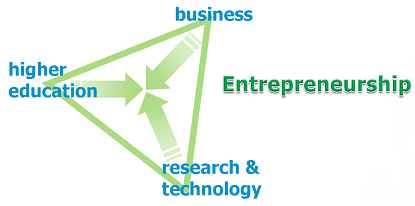
\includegraphics[width=0.8\linewidth]{picture/Knowledge_Triangle.png}
    \caption{Knowledge Triangle}\label{fig:kt}
\end{figure}

The most important constraint for our battle was setting the time frame. The starting time was decided to be the launch of Lisbon agenda at year 2000 and take into account everything until the present time, including even the possible plans for future. In this time frame, the following dates and events were the most important regarding the battle:

\subsection{March 2000: The Lisbon Agenda}
The Lisbon Agenda was a development plan for the European Union for the years 2000 to 2010. The main reason for the Lisbon Agenda was overcome the challenges that globalization and the new knowledge-driven economy brought to European Union, such as the widening skills gap especially in the information technology area\cite{3_1}. A major challenge was also the fact that the US was outperforming the European economics with its \texttt{ICT}-driven economy\cite{3_1}. Thus, the goal for Lisbon Agenda was to make \texttt{EU} ``the most competitive and dynamic knowledge-based economy in the world'' by 2010\cite{3_1}. This was intended to be reached for example through better policies for information society and R\&D and by modernizing the European social model\cite{3_1}.

\subsection{February 2005: Mid-term review of Lisbon Agenda}
On February 2005 was the publication of the mid-term review of the Lisbon Agenda, delivered by the President Barroso.
It revealed the slow progress of the goals that were set up in the Lisbon Agenda, mostly due to the lack of determined political action\cite{3_2}.
As a result, President Barroso suggested a renewed strategy with a main goal of ``delivering stronger, lasting growth and creating more and better jobs''\cite{3_3}.
One of the main focus areas was to boost knowledge and innovation for growth, and as a part of that area was the creation of European Institute of Technology (\texttt{EIT})\cite{3_3}.
The goal of the \texttt{EIT} was ``to act as a pole of attraction for the very best minds, ideas and companies from around the World''\cite{3_3}.

\subsection{February 2006: The 1st Communication}
On February 2006 the European Commission sent a first communication to the European Council, reporting that the \texttt{EU} was still failing against competing economies such as \texttt{USA} and Japan, calling for an immediate action. From the year 2000 the innovation gap between Europe, Japan and US was constantly increasing and in Europe there was a huge cultural and intellectual gap between the researchers and entrepreneurs\cite{3_4}.
The communication was also the first formal proposal for the idea, structure, organization and composition of the European Institute of Technology (\texttt{EIT}). The main argumentation for the \texttt{EIT} was that ``Europe should not only develop the three corners of its ``knowledge triangle'' (education, research and innovation), but reinforce the bridges between them.''\cite{3_4}

\subsection{June 2006: The 2nd Communication}
On June 2006, the European Commission sent a second communication to the European Council, which provided further information about aspects of the proposal and set out, where appropriate, suggestions for addressing them. They claimed that the \texttt{EIT} should be seen as one part of an integrated strategy to mobilize education, research and innovation towards the Lisbon goals, providing also support for research and innovation at the highest levels of excellence. It is remarked that the key is combining entrepreneurial mindsets and competence with excellence in technological studies\cite{3_5}.

\subsection{Launching of \texttt{KIC}s: 2010, 2014 and 2016.}
The \texttt{EIT} announced Knowledge and Innovation Communities (\texttt{KIC}s) for the purpose of integrating all three sides of the knowledge triangle. \texttt{EIT} is operated through these autonomous \texttt{KIC}s, which are located in different hubs, combining members from each dimension of the knowledge triangle. The first three \texttt{KIC}s were launched 2010 and were Climate-\texttt{KIC}, \texttt{EIT} Digital (previous \texttt{EIT} \texttt{ICT}) and \texttt{KIC} InnoEnergy. Other two \texttt{KIC}s, \texttt{EIT} Health and \texttt{EIT} Raw Materials were launched 2014. Furthermore, two more \texttt{KIC}s, \texttt{EIT} Food and \texttt{EIT} Manufacturing, are to be established in 2016\cite{3_8}\cite{3_9}.

\subsection{Horizon 2020}
Horizon 2020 is the biggest \texttt{EU} Research and Innovation programme with nearly 80 billion euros of funding available over 7 years (2014 to 2020)\cite{3_6}. The \texttt{EIT} will contribute strongly to the objectives of Horizon 2020 and is also funded by the Horizon 2020 programme\cite{3_7}.


\section{Do we need \texttt{EIT}?\ YES}\label{sec:EIT-Yes}
The \texttt{EIT} is the \texttt{EU}'s initiative to integrate the three edges of the Knowledge Triangle. The \texttt{EU} believes that a successful integration and sharing of knowledge, information and skills is essential in order to create the jobs and growth opportunities that Europe seeks. This is because, according to \texttt{EIT}, excellent researchers, students and entrepreneurs working in isolation are much less efficient in delivering the results needed and wanted by the market and consumers.

\textbf{Without a change in direction the innovation gap between Europe and the other countries will keep increasing.} Even though efforts are being made to help minimize said gap, more help/support is still needed.

Another confirmation of how important the knowledge triangle is comes from \texttt{EURAB}, European Research Advisory Board. The successful implementation of the Lisbon strategy, states \texttt{EURAB} in its Second Opinion on the \texttt{EU} proposal for \texttt{EIT}, requires the intimate linking of the three pillars of modern economy, namely: education, research and innovation. It is true that \texttt{EIT} alone will not solve the problem and that other important issues must be tackled. In particular, reform of taxation systems, increasing the availability of venture capital, reforming the intellectual property right system. Still, \texttt{EIT} is an important contribution to fill the innovation gap\cite{4_1}.


But how exactly does the \texttt{EIT} achieve its mission? This is where the \texttt{KIC}s come into play. \texttt{EIT} takes the three pillars of the Knowledge Triangle and integrates them in the so-called Knowledge and Innovation Communities (\texttt{KIC}s). Each \texttt{KIC} has been created with a major European social and economic challenge in mind and their goal is to form creative partnerships (large and small, local and global) between the private, public and academic sectors in order to drive innovation towards defined action lines that will help them solve their challenges.

It is also to be noted that \texttt{KIC}s are autonomous  entities that are only partially funded by the \texttt{EIT}.\ In fact, there is a leverage factor of 4: more than 80\% of the \texttt{KIC}'s overall budget comes from external sources and for every euro invested from the \texttt{EU} budget, a higher investment is triggered from other sources, such as governments and private partners\cite{4_2}.


For the business pillar, the \texttt{KIC}s offer services to entrepreneurs to help them build their business. For example, the Climate \texttt{KIC}, whose goal is to drive innovation in climate change, offers an 18-month program called Accelerator in which it gives start-ups access to its network, business coaches and funding. This helps entrepreneurs to deliver cleantech start-ups to the market that can attract external investments, and in turn the entrepreneurs help to make the world a greener place, successfully making progress towards the \texttt{KIC}'s goal\cite{4_3}.

The research pillar gets boosted by a \texttt{KIC} when they support PhD candidates in research labs and manage to boost their innovative power. These students will also become an accelerator for additional funding, collaborative research and international collaboration. The \texttt{KIC} will also help them turn research results into products and services that can generate revenue.

The \texttt{EIT} supports the education pillar with its Master and PhD Schools. They believe Europe needs a new generation of professionals with excellent knowledge but also with the capability to transform ideas into products and services. They have created programmes in collaboration with excellence universities which greatly focus in enhancing its student's innovative and entrepreneurial capabilities through a series of courses, summer schools and thought-provoking talks and seminars.

Before the \texttt{KIC}s, efforts to increase Europe's innovation power were already being made. The Technical University of Berlin created the TU Berlin Centre for Entrepreneurship which focuses on creating a successful innovation and entrepreneurship environment.
The centre's co-director, Agnes von Matuschka, states that 50\% of their efforts are made towards encouraging students and researchers to take an entrepreneurial path and mentions how universities in countries like US or Israel do not need this work because the interest in such path is already there.
Even if actions are already being taken by excellence universities like TU Berlin to tackle the innovation gap between Europe and the rest of the world, they can significantly benefit from the \texttt{EIT}.\
By being involved in the Digital and Climate \texttt{KIC}'s, Jan Kratzer, chair for entrepreneurship and innovation at TU Berlin and co-director of the Centre for Entrepreneurship, confirms that they have been able to achieve closer partnerships with the industry sector\cite{4_4}.

Fostering an environment to facilitate innovation is exactly what \texttt{EIT} is about: creating the \textbf{ecosystem} to re-launch Europe. \texttt{EIT} provides the institutional framework to coordinate the required knowledge and talents. In effect, \texttt{EIT} will have a \textbf{networking function}.

The \texttt{EIT} will benefit the whole Europe by connecting the best European universities with the best people around the world. One of the key point of the \texttt{EIT} programme is in fact the \textbf{brain gain}: the best international students will be attracted to study in Europe and will likely stay here, create start-ups and generate business. Thus, when \texttt{EIT} support is distributed to networked universities, more European and international people will benefit for that support. Basically, \texttt{EIT} increases the innovation and knowledge capacity of Europe; exactly what \texttt{EU} was looking for in the Lisbon Agenda.


\section{Do we need \texttt{EIT}?\ NO}
When the \texttt{EIT} was born as a brainchild of Jos\'e Manuel Barroso, the president of the European Commission, it was met with no opposition. According to Jan van den Biesen speaking for Philips Research, it was a question of how \texttt{EIT} should be implemented, but not whether it was needed at all\cite{5_5}. As if there were no alternatives in creating this bureaucratic monster that now sits on the back of Europe's professors, researchers and students alike. The problem of the European Union's lack of innovation and lagging behind the US could be solved by other means, without creating additional hoops for the universities to jump through.

In economics, a white elephant is a project that devours your resources, produces very little in return and still you cannot get rid of it. According to its critics, the \texttt{EIT} is a white elephant for the \texttt{EU}. It gobbles up money, human resources and, most importantly, time.

The \texttt{EIT} tries to centralize innovation by setting up artificial, arbitrary projects to spend its funding on and passes these projects on to universities. It seems that they had a solution in mind for which they are looking for a problem fit for it. This phenomenon is called ex-post justification, it is thinking backwards. The \texttt{EIT} has not yet succeeded with its initial plans. For example, in February 2006 it was mentioned that the \texttt{EIT} should give to their students a European Degree\cite{5_4}. However, from June 2006, this was no longer heard in their communication circles, since they started talking about a double degree system instead, where the students get their degrees from both the entry and the exit Universities with a label of ``\texttt{EIT}''\cite{5_3}. This label does not have any actual value in itself and is only a nice-sounding name which the future employer may, or may not, care about.

Another goal for \texttt{EIT} is to bring closer, the so-called Knowledge Triangle: Education, Research and Innovation; is not that something Universities are already doing? Although they are traditionally centres of education, they also have research groups and innovation centers. Universities curriculum contents are usually developed in consultation with business, increasingly intertwined for funding reasons. Several companies are in contact with universities and have contract with research groups in which they ask the researcher to develop products and so on.

\texttt{EIT} is certainly not frugal with its spending, as they organize several events, such as summer schools. They do accommodate their students in 4-star hotels. They also seemingly spend a fortune on marketing, coming up with fancy names for their projects, while maybe, at least from an ethical and educational point of view, they could spend the money more wisely. Are all these costs really necessary? It is important to remember that such money comes from the \texttt{EU} funds, which is taxpayers money paid by all across Europe. While spending money on education is not a bad idea, maybe it would serve our continent better if the money did not end up in hotel and restaurant managers' hands.

Coming to the education aspect, \texttt{EIT} often rebrands courses already existing at the member universities. For example, a local computer science student at the University of Trento (UNITN) can enrol for all the courses that are meant for \texttt{EIT} Digital students. UNITN, and the other member universities, already offer extensive courses in English, and enroll international students. The \texttt{EIT} has only created more bureaucracy and there are a lot of infrastructural problems that requires a huge amount of money. Within this complex structure, also the students have problems. For instance, an \texttt{EIT} student from the US who did not get the scholarship, paid for all his classes as well as living costs while spending his second year in Paris, where he found out that most of his classes were only in French. He posted his story on Facebook as a warning for future \texttt{EIT} students.

Our alternative is a scheme called Excellent Universities. In our opinion, Europe's best Universities know what they are doing. They are already filled with researchers and students full of innovative ideas, but they just need more funds to realise their potential. Excellence University Schemes are already at work in several European countries, such as Germany and France. It is only needed to direct what we have at institutions that have proven their work, at universities that have demonstrated their value in the past and have good ideas about the future. \texttt{EIT}'s favourite buzzword innovation is only one half of Europe's problems: an aspect that \texttt{EIT} seems to forget is technology diffusion. The concept refers to how widely a new technology entering society is spread. It is not enough just to help its birth, it has to be adopted to people's everyday lives.

The idea is that the universities excluded from the excellence programmes need to tackle the problem of general higher education. It is not possible to create a knowledge-based society by only focusing on the top 10. The excellence level universities can house advanced research and innovation, while the applied universities could create a future workforce comprised of people confident in their knowledge and usage of technology. This kind of partitioning would actually help to close the gap that already exists between people with different social and economical backgrounds. On the other hand, the greatest benefactor of an educated society is the business world, the companies looking for workforce. These companies should fund their future worker's studies as much as possible. This needs, of course, a huge amount of trust from both sides. A differentiated, self-aware and honest higher education system could help the companies to decide, which programmes they should fund. It could be possible to turn the applied universities into ``buyer's markets of talent and knowledge''. With companies actively taking part in higher education, students and their professors could focus on actual real-world problems, looking for solutions together. When the students finish their studies, they already have years of experience and can move around confidently in the business world.

None of these ideas are new, nor are they mind-blowingly original and shocking. The point is, all the tools needed to reinvent Europe are already in our hands. Europe has top-ranking universities already in countries such as Britain, Germany and the Nordic countries\cite{5_2}. There is no need to create another bureaucratic agency that stands between researchers and their funding. \texttt{EIT} sounds like an easy solution, a flashy PR manoeuvre with a fine sounding name, but it is not really an answer to the existing problem.

Educational reform is not easy, on the contrary, in our professor's words, it is too ``complex''. But by taking into account the universities capabilities and by helping them to realize their full potential with much needed funding, they can become flagships of European Excellence.
Europe can take back the leading position not by mindlessly copying the \texttt{MIT}, but by taking the initiative. Europe should utilize the diverse cultures, the different perspectives, the traditions and fresh ideas and work together to create a new world of intellectual prosperity.

\section{European Excellence on the Rise}
Research and development make a significant contribution to the growth of the European economy and Europe's accomplishments in areas such as science and technology is considered to be some of the best by the rest of the world. Many of the most appraised researchers are European as they stand out for their excellent work, most notably in the mathematical, physics, chemistry, and engineering fields.

Scientific research in Europe is based on the most re-known European universities and scientific institutions. If Europe already excels in research and development works and has some of the most renowned institutions, such as European Organization for Nuclear Research, Institute for Environment and Sustainability, and others, the following question arises: \textbf{Why did the \texttt{EU} Commission propose a new Institute?}

After the disappointing conclusions of the Lisbon Agenda's Midterm Review in 2005, the then \texttt{EU} Commission President, Jose Manuel Barroso, presented the idea to create the European Institute of Technology (\texttt{EIT}) to help achieve the growth in innovation that Europe was seeking with this Agenda. It was instantly debated about how such institute should be implemented, not about whether it was needed at all.

The European Commission's analysis is that the continent suffers from insufficient quality and usability of its high quality research output, gaps between the creation of knowledge and its commercial exploitations, and a general developing a discovery in the laboratory into a new product or service.\cite{6_1} With this analysis, the basis for creating the \texttt{EIT} is reasonable: Europe must do more to address weaknesses in the \textbf{Knowledge Triangle} of education, research and innovation, particularly if it wants to become the world's leading knowledge-based economy\cite{6_1}. The \texttt{EIT} is a distributed system. It operates in \texttt{KIC}s: Knowledge and Innovation Communities distributed across Europe, with its main headquarters in Budapest, Hungary. Each of these \texttt{KIC}'s address a major European social and economic challenge and set up a set of action lines to tackle it.

Like stated in Section~\ref{sec:EIT-Yes}, the \texttt{EIT} supports the education pillar of the Knowledge Triangle through a partnership with some of the best European universities and together have created programmes which focus on enhancing its European student's innovative and entrepreneurial  potential. But what if the problem could be solved by other means, without creating an institute that would add more hoops for the universities to jump through. Maybe, instead of setting up new authorities that gobble up resources, those resources could be directed straight towards universities  that have already proven their worth.

Although some European education and research institutions are excellent, today some are isolated from the business world and do not work together to create market-driven solutions and innovation. To address this problem, one of the proposed schemes is called: \textbf{Excellence University Scheme} that are already at work in several European countries. For example, The Excellence Initiative in Germany, which shares many of its goals with the \texttt{EIT}: creating a nurturing environment for research and university work, to bring institutions and disciplines together, and to promote international cooperation. With this strategy, Germany aims to become an internationally renowned beacon of innovation, but its method could be applicable for the whole \texttt{EU}\cite{6_3}. The Excellence University Scheme believes that when resources are scarce, efforts should be directed at institutes that proven their value in the past, and have clear and original ideas about the future.

It is debated that the \texttt{EIT} tries to \textbf{centralize innovation} by setting up artificial, arbitrary projects to spend its funding on, and passes these projects onto its partner universities, just as if the institution had a solution in mind, and now they are looking for a problem that fits. The Excellence University Scheme states that Europe's best universities know what they are doing, they are already filled with researchers and students full of innovation ideas, they just need the extra kick, the extra funding to take off and reach their full potential.

One of the drawbacks of the Excellence University Scheme is selecting the recipients of \texttt{EU} funding. It is not an easy task because of the evident rivalry between European universities, where many claim to be the best. And they very well are some of the best, in their respective countries, but when thinking about an international setting, national pride should be put aside. It cannot be about politics, and power: it is about education, and Europe's future is at stake\cite{6_4}.

With funding being directed to towards the \texttt{EIT} and then on to the universities through their established partnership, the budget will be distributed among more universities, but each of them will use this funding to work towards the established \texttt{EIT} goals, depending on the \texttt{KIC} the university belongs to and the main challenge and action lines they support. Distributed efforts will manage to achieve a common goal. Also, it should not be forgotten that, through the strategies implemented to support the business pillar, \texttt{EIT} develops partnerships with the industry and is capable to obtain more funding.

Distributing the European Union's funding is a tough decision, but efforts need to be concentrated to make a real difference, because otherwise the help is spread too thin. One of the objectives of the \texttt{EIT} is to use its funding to be able to create an easier link between students, research centers and business partners. But the \texttt{EIT} is scattered, and with its budget of a few hundred millions of euros it can hardly challenge the \texttt{MIT}, the institution it tries to imitate.

On the other hand, \texttt{EIT}'s distributed network is a great way to raise money from the companies around Europe. This concept can be clarified through the following example: if \texttt{FIAT}, a big Italian industry, needs to develop a new kind of technology for its industrial needs, is it more simple for them to contact, work and fund the research of an Italian university or of an ``excellent'' one in the north of Europe? The closer, the better; distances still matter.

In the end, there is the need to \textbf{strike the right balance} between the two big concepts: \textbf{distribution and centralization}. The structure should be distributed enough, so that you can reach every part of Europe, both to achieve technological distribution and to raise more fundings from all the different sources (industries, government, etc.) across Europe. Yet, the structure should be centralized enough so that the funding is still sufficient to really unlock the possibility to compete in research and innovation with the very best universities worldwide.

The other key word is \textbf{collaboration}. Competition is a wonderful engine to drive towards innovation, but if the European universities are able to envision themselves as a unique entity instead of enemies, if they are able to really share their knowledge instead of fighting for it, Europe should be really leading the way into future. By achieving this, universities could exploit a new way to take advantage of the cultural diversity that is present in Europe. In which other part of the world do they have the ``funky'' Italians, the ``methodical'' Germans and the ``precise'' English/Scandinavians? How many different kind of ideas could be obtained from these many different kinds of people? These ideas should be shared, discussed, improved, implemented, and used to make money out of them.

To unlock this potential there is still a couple of ``elephants in the room'': \textbf{bureaucracy and consistency}. Bureaucracy still poses too many obstacles between the different universities, and in particular between sharing people and ideas. If a student tries to apply for example to \texttt{EIT}, it is not an easy task. Student has to take a lot of time and effort to fill the application forms and get all the needed documents and diplomas from the university and other organizations to be eligible for applying. The inconsistency of needed documents for each university makes it even harder to be sure that the application will not be rejected because of missing documents. Moreover, if a student has a good idea and a university has the perfect network to develop it, how long would it take to him to achieve his goals? These are barriers that need to be taken down and this process goes together with consistency. There is a big need of uniforming the universitary system in Europe, which could lead to a thinner bureaucracy and a better network of universities.

\section{A step forward}
The launch of an \texttt{EIT} was an attempt to overcome the fact that Europe was still falling short against US and other economies in terms of innovation. Thus, the European Commission decided to accelerate the process of innovation making and established the \texttt{EIT}. There was no doubt that the problems Europe was facing needed to be solved, but there was not enough discussion whether the \texttt{EIT} was the right answer for these problems. Hence, the \texttt{EIT} got a lot of criticism for not being a universally agreed answer to the problems but rather a quickly crafted solution.

It must however be taken into account that every innovative move is a risk and establishing an institute like the \texttt{EIT} to face the challenges Europe has is an innovation itself. This means that it also has a risk of failure. If you think about it, the risk increases because of the new random variable called \texttt{EIT}. Nevertheless, the \texttt{EIT} has been growing to now be one of the leading factors to help Europe build its innovative potential. So can we say that the risk has been worth taking? It is very hard to analyze such complex system as the \texttt{EIT} is. Moreover, it is impossible to make a precise prediction in framework of international society. This kind of  uncertainty can be seen more precisely only within a few additional years of the \texttt{EIT} progress.

Despite all the initial criticisms, concerns and objections, the \texttt{EIT} is now in place and its \texttt{KIC}s are already running. The \texttt{EU} Commission's plan was to create a European institution unique, different from any \texttt{EU} initiative currently implemented and that manages to exploit the relationship between education, research and companies. This is exactly what \texttt{EIT}'s mission is about: it tries to combine, as mentioned before, the three sides of the Knowledge Triangle. This is definitely a big step into the future of Europe and in this lies the real challenge of the current policy.

The results of the \texttt{EIT} are still debatable. \texttt{EIT} has brought together many of the excellence universities around Europe and also raised many other universities status by accepting them as part of the \texttt{EIT}. The \texttt{EIT} community has gotten a good amount of attention internationally with relatively small budget and especially the entrepreneurial results of the students have been successful. However, the amount of innovations coming through the \texttt{EIT} still remains small and the real effect for participating universities is still unclear, since the \texttt{EIT} programs have been up and running only for a few years.

It is true that the budget the \texttt{EIT} currently has and how it has to be distributed to a network of partner universities is barely enough to compete with the much larger budget of \texttt{USA}'s \texttt{MIT}. Spending the amount of the \texttt{EIT} budget to fund the already existing few excellence universities of Europe might have a bigger impact on the rankings of the universities, but it might not help Europe to achieve its goals in a global scale. Spreading the budget of the \texttt{EIT} across the participating universities means that the impact to individual universities in Europe is not as significant. However, that way the funding reaches more European universities that can help and work together to improve Europe's innovation capabilities.

In order for such a model to be able to bring positive results, the \texttt{EU} Commission should be aware that the \texttt{EIT} must be sufficiently attractive for universities, research institutions and companies, since their participation is a crucial factor to achieve its goal of strengthening innovation in Europe. Hopefully, the opportunity to influence the direction of research should be a sufficient attractive factor for the private sector. Worries arise in considering that the current program does not emphasize explicitly that the main objective of the \texttt{EIT} is innovation.

Research is already one of Europe's strengths, innovation is the missing link. MEP Jerzy Buzek reiterated that the \texttt{EIT} must not subtract resources from other innovation and research programmes, nor will it try to compete with other universities in Europe, he stated that ``it is not a new university, it is a quite different idea all together''\cite{7_1}. These concerns are reasonable if we consider the possibility that universities, research institutes and companies truly allow that their best teams become legally divorced from their organization for at least a decade.

The first step taken by the Commission is positive, but the debate based on a full understanding of the innovation process as well as an explanation of the reasons why this system is making a difference, has just started.

\textbf{So, will the \texttt{EIT} be the solution}? Will the \texttt{EIT} work? Maybe yes. The \texttt{EIT} could become a novel European solution to various structural problems. It could really create innovation and exploit European resources connecting students, researchers and businessmen. Or perhaps it will just become a weak compromise to fulfill a short-term political need, without addressing the core problem. The \texttt{EIT} is a great step forward but not entirely the solution of the Europe's innovation gap problem. If it was so, we would not have any need to have a battle about it, and we really hope it would be the case in the near future.

%\clearpage
%\bibliographystyle{plain}
\bibliographystyle{acm}
\bibliography{bibliography}

\end{document}
